%==========================================================================
% Artigo científico UNESC (TCC final)
% Estrutura NOVA derivada do main.tex do projeto (knowledge/fontes/overleaf/main.tex).
% O preâmbulo, o título, os autores e os rodapés são idênticos ao original.
% Acréscimos em relação ao original: pacote xcolor e macro \PENDENTE
% (marcações em vermelho para o que depende de dados, da orientadora ou do autor)
% e os \input das seções.
%
% Template original:
% v0.0 versão em 20/09/2023 por Marlon Oliveira
% v1.0 versão em 25/06/2025 por Marlon Oliveira
%==========================================================================

%==========================================================================
% Pacotes utilizados pela UNESC - não delete as linhas abaixo
%==========================================================================
\documentclass{UNESC}
\usepackage[T1]{fontenc}
\usepackage[utf8]{inputenc}%\usepackage[latin1]{inputenc}
\renewcommand{\rmdefault}{phv} % Arial
\renewcommand{\sfdefault}{phv} % Arial
\usepackage[brazilian]{babel}
\usepackage{graphicx}
%\usepackage{subfigure}
\usepackage{hyperref}
\usepackage{quoting}
\usepackage[labelsep=none]{caption}
\DeclareCaptionLabelFormat{figuracomtraco}{#1~#2 -}
\captionsetup[figure]{labelformat=figuracomtraco, labelsep=space}
\captionsetup[table]{labelformat=simple, labelsep=space, textformat=simple}
\DeclareCaptionLabelFormat{tabelacomtraco}{#1~#2 -}
\captionsetup[table]{labelformat=tabelacomtraco}
\captionsetup{labelsep=none}
% ACRÉSCIMO 04/11/2026 (orientações fixadas do prof. Marlon): legenda com recuo
% pendente e legenda e "Fonte:" alinhadas ao início da tabela/figura.
\captionsetup{format=hang, justification=raggedright, singlelinecheck=false}
\newlength{\largurafl}
\newlength{\larguraorigfl}
% \flutuante{conteúdo}{legenda+label}{fonte}: mede a largura do conteúdo (notas com
% \linewidth valem zero na medição) e empilha legenda, conteúdo, notas e fonte nessa largura.
% ACRÉSCIMO 04/11/2026: se o conteúdo (tabela e notas) for mais largo que o texto, ele é
% reduzido para caber em \textwidth, em vez de invadir a margem direita e ser cortado.
\newcommand{\flutuante}[3]{%
  \begingroup\setlength{\linewidth}{0pt}\settowidth{\largurafl}{#1}\global\largurafl=\largurafl\endgroup
  \ifdim\largurafl>\textwidth
    \larguraorigfl=\largurafl
    \largurafl=\textwidth
    \begin{minipage}{\largurafl}#2%
    \resizebox{\largurafl}{!}{\begin{minipage}{\larguraorigfl}#1\end{minipage}}\par\vspace{0.2cm}%
    {\footnotesize #3\par}\end{minipage}%
  \else
    \begin{minipage}{\largurafl}#2#1\par\vspace{0.2cm}%
    {\footnotesize #3\par}\end{minipage}%
  \fi}
%\renewcommand{\thefigure}{\arabic{figure} - }
\usepackage{enumitem}
\usepackage{float}
\usepackage{comment}
\usepackage[hang,flushmargin]{footmisc}
\usepackage{array}
\usepackage{booktabs}% tabelas geradas por tcclab relatorio (ALINHAMENTOS.md)

% ACRÉSCIMO (único pacote novo): cores para a macro \PENDENTE
\usepackage{xcolor}
% Para conferir o texto sem as marcações, troque a definição abaixo por
%   \newcommand{\PENDENTE}[1]{}
% (o texto deve fazer sentido sem elas) e, no fim, remova as chamadas.
% Versão limpa (para a orientadora/entrega): \versaolimpatrue esconde as marcações.
% As perguntas que elas continham estão em PERGUNTAS-ORIENTADORA.md.
\newif\ifversaolimpa
\versaolimpatrue
\ifversaolimpa
  \newcommand{\PENDENTE}[1]{}
\else
  \newcommand{\PENDENTE}[1]{\textcolor{red}{\textbf{[PENDENTE: #1]}}}
\fi

\hypersetup{
  setpagesize  = false,
  colorlinks   = true,    % Colours links instead of ugly boxes
  urlcolor     = blue,    % Colour for external hyperlinks
  linkcolor    = black,   % Colour of internal links
  citecolor    = black    % Colour of citations
}
\urlstyle{same}
\usepackage{setspace}

\usepackage[alf,recuo=0.0cm,abnt-emphasize=bf]{abntex2cite}

%\captionsetup[figure]{justification=raggedright}


%==========================================================================
% Dados do artigo: título, autores e filiação
%==========================================================================
\title{BOAS PRÁTICAS DE INDEXAÇÃO E OTIMIZAÇÃO DE CONSULTAS EM SQL SERVER: UMA ABORDAGEM METODOLÓGICA BASEADA EM MÉTRICAS DE PERFORMANCE}
\author
{
   Douglas Gonçalves E Barra\footnote{Curso de Ciência da Computação, Universidade do Extremo Sul Catarinense (Unesc), Criciúma - Santa Catarina - Brasil. douglasbarra11@unesc.net},
   %Nome Completo do corientador(a)\footnote{Corientador(a), Curso de Ciência da Computação, Universidade do Extremo Sul Catarinense (Unesc), Criciúma - Santa Catarina - Brasil. email@unesc.net}
   Ana Cláudia Garcia Barbosa, Ma.\footnote{Orientador(a), Curso de Ciência da Computação, Universidade do Extremo Sul Catarinense (Unesc), Criciúma - Santa Catarina - Brasil. agb@unesc.net}
}
%==========================================================================
% Início do texto do artigo
%==========================================================================
\begin{document}

\onehalfspacing

\maketitle

% Resumo, Abstract e palavras-chave (ver README.md para ajustar ao template)
% =====================================================================
% RESUMO, PALAVRAS-CHAVE, ABSTRACT E KEYWORDS
%
% Versão mais simples possível: parágrafos com rótulo em negrito, como nos TCCs
% de exemplo (Resumo: ...; Palavras-chave: ...; Abstract: ...; Keywords: ...).
% Não depende de ambiente da classe UNESC. Se a classe oferecer ambientes ou
% comandos próprios (por exemplo \resumo{...}), troque APENAS a moldura e mantenha
% o texto. Ver README.md, seção "O que ajustar no template UNESC".
%
% Regras: até 250 palavras cada, sem citação bibliográfica, com problema,
% solução, hipótese, resultados e conclusão. Resultados e conclusão ficam
% como \PENDENTE até a execução do experimento. Ao preencher, reconferir a
% contagem de palavras (alvo: 190 a 230).
% =====================================================================

\begingroup
\singlespacing

\noindent\textbf{Resumo:} A escrita de consultas em bancos de dados relacionais figura entre as tarefas de maior esforço no desenvolvimento de \textit{software}, e o desempenho costuma ceder lugar à correção funcional. As ferramentas automáticas de ajuste de índices atuam depois que a consulta foi escrita e não orientam quem a escreve. Este trabalho propôs um \textit{framework} metodológico de quatro camadas, diagnóstico, análise, prescrição e validação, que organiza práticas de indexação e de reescrita de consultas no SQL Server. A hipótese foi que o \textit{framework} reduz em pelo menos 20\% as leituras lógicas de consultas com antipadrões de escrita. Realizou-se um experimento do tipo antes e depois sobre o conjunto de dados público Stack Overflow 2010, com 19 consultas de quatro classes de antipadrões, medidas nas formas original e otimizada quanto às leituras lógicas, ao tempo de processamento e ao tempo de execução, além do custo de escrita dos índices e da comparação com o índice sugerido pela ferramenta nativa. A redução mediana das leituras lógicas nas 17 consultas principais foi de 99,9\% (teste de Wilcoxon, $p < 0{,}001$), e 16 delas atingiram o limiar. A subconsulta correlacionada teve o menor efeito, e em uma consulta a prescrição manual não atacou o gargalo que o índice nativo encontrou. A reescrita isolada não reduziu as leituras, e um índice que não cobria a consulta a piorou. Concluiu-se que a hipótese foi confirmada para o conjunto e que o método manual e a ferramenta nativa se complementam.

\medskip
\noindent\textbf{Palavras-chave:} otimização de consultas; indexação; SQL Server; desempenho de bancos de dados; antipadrões de consulta.

\bigskip
\noindent\textbf{Abstract:} Writing queries for relational databases is among the most demanding software development tasks, and performance often gives way to functional correctness. Automatic index tuning tools act after the query has been written and do not guide the person writing it. This work proposed a four-layer methodological \textit{framework}, composed of diagnosis, analysis, prescription and validation, which organizes indexing and query rewriting practices in SQL Server. The hypothesis was that the \textit{framework} reduces logical reads by at least 20\% in queries with writing antipatterns. A before-and-after experiment was carried out on the public Stack Overflow 2010 dataset, with 19 queries from four antipattern classes, measured in their original and optimized forms for logical reads, CPU time and elapsed time, together with the write cost of the indexes and a comparison with the index suggested by the native tool. The median reduction in logical reads across the 17 main queries was 99.9\% (Wilcoxon test, $p < 0.001$), and 16 of them reached the threshold. Correlated subqueries had the smallest effect, and in one query the manual prescription missed the bottleneck that the native index found. Rewriting alone did not reduce reads, and an index that did not cover the query made it worse. It was concluded that the hypothesis was confirmed for the set and that the manual method and the native tool complement each other.

\medskip
\noindent\textbf{Keywords:} query optimization; indexing; SQL Server; database performance; query antipatterns.

\endgroup


% =====================================================================
% 1 INTRODUÇÃO (prosa, sem subseções)
% Contém: contexto, teoria mínima (Fundamentação Teórica condensada, decisão 13),
% estado da arte e trabalhos correlatos (movidos da antiga seção 2 em 05/11/2026,
% regra do prof. Marlon: só 4 seções; modelo: TCC de Mateus S. de Matos, 2026-1), lacuna, problema e hipótese, objetivos (5 específicos, um verbo
% cada), justificativa e estrutura do trabalho.
% Origem de cada trecho: ver ALINHAMENTOS.md.
% =====================================================================

\section{INTRODUÇÃO}\label{sec:introducao}

O desempenho de sistemas de \textit{software} que armazenam dados em bancos relacionais depende da eficiência com que as consultas, escritas na linguagem SQL (\textit{Structured Query Language}), são executadas. Em aplicações corporativas, problemas de indexação, estimativas incorretas de cardinalidade, isto é, do número de registros que uma condição seleciona, e planos de execução lentos tornam-se críticos à medida que crescem o volume de dados e a complexidade das consultas \cite{sirigiri2025sqlperf}.

Consultas mal estruturadas, ausência de índices adequados ou uso incorreto dos índices existentes resultam em operações ineficientes, como as varreduras completas de tabela, que percorrem a tabela inteira mesmo quando apenas uma fração dos registros é necessária. Um número elevado de leituras lógicas, isto é, de páginas de dados lidas da memória durante a execução de uma consulta, indica essas varreduras e costuma decorrer da falta de índices \cite{rusanu2014perf}.

Para executar uma consulta, o SQL Server, sistema gerenciador de bancos de dados relacionais, conta com um componente interno, o otimizador de consultas, que escolhe a forma mais eficiente de acessar os dados. Em vez de executar a consulta exatamente como foi escrita, o otimizador a transforma em um plano de execução, uma sequência de operações físicas, como varreduras, buscas e junções (combinação de registros de tabelas diferentes), que descreve como os dados serão acessados \cite{fritchey2018plans}. A escolha do plano depende das estatísticas que o sistema mantém sobre a distribuição dos valores de cada coluna, as quais estimam quantos registros atendem a um filtro. Quando essas estimativas são imprecisas, por estatísticas desatualizadas ou por distribuições de dados irregulares, o otimizador pode escolher planos inadequados \cite{leis2015good, han2022cardest}.

O índice é uma estrutura auxiliar que organiza os valores de uma ou mais colunas para que o sistema localize registros sem percorrer a tabela inteira. Sua eficácia depende da seletividade da coluna indexada, a proporção entre valores distintos e registros: identificadores únicos têm alta seletividade e se beneficiam do índice, enquanto campos com poucos valores possíveis tendem a oferecer ganho reduzido \cite{fritchey2018qpt}. Em índices compostos, definidos sobre mais de uma coluna, a ordem das colunas determina o aproveitamento: se a consulta não filtra pela primeira coluna, o sistema recorre com frequência a uma varredura completa \cite{fritchey2018qpt}. O índice tem ainda um custo de manutenção, pois cada inserção, atualização ou exclusão precisa atualizá-lo, e o índice escolhido influencia o tempo de acesso e o de inserção \cite{saidu2024indexing}. Além dos índices, a forma como a consulta é escrita determina o plano resultante. Chamam-se antipadrões os padrões de escrita que retornam o resultado correto, mas levam a operações ineficientes \cite{karwin2010antipatterns}. Este trabalho tratou de quatro: a aplicação de funções sobre colunas usadas em filtros, que impede o uso eficiente do índice; a subconsulta correlacionada, reexecutada para cada registro da consulta externa e que pode ter tempo de execução quadrático em relação ao número de registros \cite{neumann2025unnesting}; a seleção desnecessária de colunas, que obriga o sistema a buscar na tabela base os dados que o índice não contém \cite{karwin2010antipatterns, fritchey2018qpt}; e a varredura completa por falta de índice, em que o sistema lê todas as páginas da tabela para encontrar poucos registros \cite{fritchey2018qpt}.

Apesar da relevância do tema, a escrita de consultas é uma tarefa exigente. \citeonline{dacosta2023sql} analisaram relatos de problema (\textit{issues}) de 20 projetos de código aberto da Apache Software Foundation e observaram que a mediana do tempo de resolução dos relatos relacionados a SQL foi de 25.897 minutos, contra 10.161 minutos nos demais, e que 53\% dos relatos relacionados a SQL receberam classificação de esforço percebido nas categorias mais altas da escala, contra 14\% nos demais, embora os próprios autores qualifiquem como pequena a diferença no tempo de resolução. Esse esforço favorece que a correção funcional, isto é, a capacidade de retornar os resultados esperados, prevaleça sobre o desempenho e que antipadrões como os descritos acima apareçam nas consultas.

Para situar este trabalho, foram analisadas pesquisas internacionais e nacionais sobre otimização de consultas e ajuste de índices, que se concentram na automação.

\citeonline{leis2021cost} propuseram um modelo que considera a carga de trabalho e o \textit{hardware} para determinar a configuração ideal de instâncias de computação em nuvem em sistemas de processamento analítico, observando que desempenho e custo podem variar em ordens de grandeza conforme a configuração escolhida. Sob a ótica deste trabalho, a limitação é que a decisão ocorre na camada de infraestrutura e não aborda a indexação nem a escrita da consulta em ambientes transacionais.

\citeonline{gretscher2025vldb} compararam abordagens de otimização de consultas, a dividida (\textit{split}), a holística e a híbrida, em um sistema de pesquisa, avaliando o tempo de otimização e a qualidade do plano de execução resultante, e propuseram uma estratégia híbrida. O estudo concentra-se na construção do plano pelo otimizador, ou seja, na perspectiva de quem desenvolve sistemas gerenciadores de bancos de dados, e não propõe método para quem escreve as consultas.

\citeonline{wu2024indextuning} elaboraram um levantamento sobre o ajuste automático de índices, que organiza as técnicas em pré-processamento, estimativa do benefício dos índices e seleção de índices, e discute sua aplicação em produtos comerciais e de código aberto. O levantamento é abrangente quanto às técnicas, mas não propõe um modelo estruturado que o desenvolvedor aplique de forma manual e iterativa ao escrever e revisar consultas.

\citeonline{brucato2024wred} propuseram a redução da carga de trabalho (\textit{workload reduction}) como técnica complementar para acelerar o ajuste de índices, diminuindo o tempo de cada chamada ao otimizador com índices hipotéticos sem afetar de modo relevante a qualidade do ajuste. Assim como o levantamento anterior, o trabalho mantém o foco na automação sobre uma carga de trabalho já existente, etapa posterior à escrita das consultas. \PENDENTE{confirmar com a orientadora se a autoria de pesquisadores da Microsoft em Brucato et al. (2024) é compatível com a regra de não citar a Microsoft (decisão 24)}

No contexto nacional, \citeonline{marins2021outertuning} apresentaram o \textit{Outer-Tuning}, \textit{framework} extensível, baseado em ontologia de domínio, para a sintonia semiautomática de bancos de dados relacionais. \citeonline{perciliano2021ondbtuning} detalharam a inferência de ações de sintonia com a ontologia OnDBTuning e a avaliaram na recomendação de índices. \citeonline{oliveira2022autonomic} propuseram um método automático para gerar e selecionar combinações de ações de sintonia, com soluções mais eficientes do que as locais independentes. Mais próximo da etapa de prescrição deste trabalho, \citeonline{araujo2014aresql} propuseram o ARe-SQL, abordagem automática e não intrusiva de reescrita de consultas SQL baseada em 11 heurísticas, com ganhos de até 92,5\% em alguns casos. A Tabela~\ref{tab:correlatos}, na seção~\ref{sec:comparacao}, resume os trabalhos e a lacuna de cada um.

Entre os métodos de ajuste automático de índices, parte considera apenas a recuperação de dados, sem o impacto das modificações, e outra parte inclui o custo de manutenção dos índices \cite{wu2024indextuning}. Nos planos coletados neste trabalho, a sugestão do recurso de índices ausentes do SQL Server traz as colunas e o impacto estimado na consulta, e não o custo que o índice impõe às operações de escrita.

A lacuna está em que, entre os trabalhos analisados, as soluções atuam sobre a consulta já escrita e visam à automação, e não foi encontrado método que oriente o desenvolvedor durante a escrita da consulta, relacione antipadrões a estratégias de indexação e verifique o efeito por métricas objetivas. O problema de pesquisa foi, portanto, como sistematizar boas práticas de indexação e de escrita de consultas em SQL Server de modo que seu efeito seja verificável. Formulou-se a hipótese de que a aplicação do \textit{framework} proposto reduz em pelo menos 20\% as leituras lógicas de consultas com antipadrões de escrita. \PENDENTE{confirmar com a orientadora o limiar de 20\%, que é parametrizável; o mesmo valor aparece no Resumo, no Abstract, nos objetivos, na seção 3 e na Conclusão} Para investigá-la, este trabalho propôs um \textit{framework} metodológico de quatro camadas sequenciais, diagnóstico, análise, prescrição e validação, fundamentado na literatura e validado em um experimento do tipo antes e depois com um conjunto de dados público.

O objetivo geral é propor um \textit{framework} metodológico de quatro camadas para a otimização de consultas em SQL Server, tendo como critério de eficácia a redução mediana de pelo menos 20\% nas leituras lógicas de consultas com antipadrões de escrita. Os objetivos específicos são revisar trabalhos correlatos qualificados sobre otimização de consultas e ajuste de índices, com as limitações de cada um consolidadas em quadro comparativo; catalogar quatro classes de antipadrões de escrita, cada uma com ao menos quatro consultas de teste nas versões original e otimizada; definir o modelo do \textit{framework}, com critérios verificáveis em cada camada e um limiar de melhoria significativa; executar o experimento antes e depois sobre o conjunto de dados público Stack Overflow 2010, com 20 repetições por consulta no cenário quente e 8 no frio; e mensurar a variação percentual das leituras lógicas, do tempo de processamento e do tempo de execução entre as versões original e otimizada, por antipadrão.

O trabalho se justifica pela contribuição de um método sistematizado, de aplicação manual e iterativa, que explicita a relação entre a escrita da consulta, a indexação e o desempenho, e que submete cada recomendação à verificação por métricas objetivas e à medição do custo de escrita. Entre os trabalhos analisados, o ineditismo está em reunir, em um único procedimento verificável, a identificação de antipadrões, a análise dos índices existentes, a prescrição e a validação. O SQL Server foi escolhido por oferecer recursos nativos de diagnóstico de desempenho, como o \textit{Query Store}, repositório que armazena o histórico dos planos de execução e permite identificar regressões de desempenho ao longo do tempo \cite{fritchey2018qpt}, e por adotar o T-SQL, dialeto da linguagem SQL próprio desse sistema.

Este artigo está organizado em quatro seções, contando esta introdução. A seção~\ref{sec:mm} descreve os materiais e métodos: o \textit{framework}, o catálogo de antipadrões, os dados e o ambiente, o delineamento, os procedimentos e a análise dos dados. A seção~\ref{sec:rd} apresenta e discute os resultados, e a seção~\ref{sec:conclusao} traz a conclusão, as contribuições, as limitações e os trabalhos futuros.


% Trabalhos correlatos: movidos para o fim da Introdução (texto) e para a seção 4.5 (Tabela 1)
% em 05/11/2026; a regra do prof. Marlon admite só 4 seções. Original em versoes/2026-11-05-antes-correlatos/.

% =====================================================================
% 3 MATERIAIS E MÉTODOS
% Reorganiza Trabalho Proposto + Metodologia + Recursos Necessários nas quatro
% partes de Lakatos e Marconi (objeto de estudo, delineamento, procedimentos,
% análise dos dados).
%
% REGRA DE OURO: nada é declarado como feito se ainda não foi executado.
% - Passado: decisões de projeto e o ambiente já montado (fatos verificados em
%   knowledge/13-infra-sqlserver-docker.md).
% - Tudo que depende do experimento (números, versões finais, resultados de
%   comandos) está como \PENDENTE.
% - Subseções 3.5 a 3.7: o texto descreve o protocolo DEFINIDO, em presente;
%   ao executar o experimento, reler e converter os verbos para o pretérito
%   (ver \PENDENTE no início de 3.5).
% =====================================================================

\section{MATERIAIS E MÉTODOS}\label{sec:mm}

Esta seção apresenta a contribuição do autor e as informações necessárias para reproduzir o experimento, em quatro partes: o objeto de estudo (subseções~\ref{sec:framework} a~\ref{sec:materiais}), o delineamento (subseção~\ref{sec:delineamento}), os procedimentos (subseção~\ref{sec:procedimentos}) e a análise dos dados (subseção~\ref{sec:analise}).

\subsection{Caracterização da pesquisa e hipótese}\label{sec:caracterizacao}

Esta pesquisa caracteriza-se, quanto à sua natureza, como aplicada, uma vez que tem como finalidade a produção de conhecimento direcionado à solução de um problema prático identificado no desenvolvimento de sistemas que dependem de bancos de dados relacionais. Quanto aos objetivos, classifica-se como exploratória e descritiva, na medida em que busca aprofundar a compreensão do tema por meio da revisão bibliográfica e descrever de forma sistemática o comportamento das consultas antes e depois da aplicação do \textit{framework}. Quanto aos procedimentos técnicos, combina revisão bibliográfica e desenvolvimento experimental, conduzido por testes práticos em ambiente controlado de banco de dados. \PENDENTE{confirmar a classificação da pesquisa com a orientadora: a taxonomia da disciplina não traz \textquotedblleft aplicada\textquotedblright{} como natureza, e \textquotedblleft exploratória\textquotedblright{} indica ausência de hipótese, que o artigo formula (decisão 21)}

A hipótese operacional é que as recomendações das camadas de análise e de prescrição reduzem em pelo menos 20\% a mediana das leituras lógicas das consultas com antipadrões (seção~\ref{sec:introducao}). O custo de escrita dos índices criados foi incluído para verificar se o ganho na leitura se mantém.

\subsection{O \textit{framework} de quatro camadas}\label{sec:framework}

O \textit{framework} foi concebido como um processo iterativo de quatro camadas sequenciais (Figura~\ref{fig:framework}): a saída da camada de validação pode retroalimentar uma nova rodada de diagnóstico, o que permite refinar as consultas e os índices.

\begin{figure}[H]
\centering
\flutuante{%
\resizebox{\textwidth}{!}{%
\fbox{\parbox[c]{3.6cm}{\centering\textbf{1. Diagnóstico}\\[2pt] antipadrões e evidências no plano de execução}}
$\rightarrow$
\fbox{\parbox[c]{3.6cm}{\centering\textbf{2. Análise}\\[2pt] índices existentes, seletividade e custo de escrita}}
$\rightarrow$
\fbox{\parbox[c]{3.6cm}{\centering\textbf{3. Prescrição}\\[2pt] reescrita da consulta e criação ou ajuste de índice}}
$\rightarrow$
\fbox{\parbox[c]{3.6cm}{\centering\textbf{4. Validação}\\[2pt] três métricas, custo de escrita e comparação com o índice nativo}}
}%
}{\caption{Camadas do \textit{framework} e ciclo de iteração}\label{fig:framework}}{Sem melhoria significativa ou com efeito colateral negativo, o processo retorna à camada 1.\\[0.1cm]Fonte: Do autor.}
\end{figure}

A camada de diagnóstico identifica, em uma consulta existente, antipadrões de escrita associados a operações ineficientes, a partir do plano de execução: varreduras completas de tabela, funções aplicadas a colunas filtradas e subconsultas correlacionadas em contextos em que uma junção seria mais adequada \cite{neumann2025unnesting, karwin2010antipatterns}. O resultado é um conjunto de evidências objetivas que fundamenta as camadas seguintes.

A camada de análise examina as evidências em conjunto com os índices já existentes nas tabelas, avalia a seletividade das colunas usadas nos filtros e nas junções e determina se a causa da ineficiência é a ausência de um índice adequado ou o uso inadequado de um índice existente \cite{fritchey2018qpt}. Além do ganho estimado na leitura, considera o impacto potencial de um novo índice sobre as operações de escrita \cite{saidu2024indexing}.

A camada de prescrição traduz a análise em recomendações objetivas: a reescrita da consulta, que elimina o antipadrão; a criação ou o ajuste de índices, com a ordem das colunas justificada pela seletividade; ou ambas. As recomendações são diretrizes específicas e tecnicamente justificadas, e não sugestões genéricas.

A camada de validação verifica se as recomendações resultaram em ganho de desempenho. Compara as três métricas, leituras lógicas, tempo de processamento e tempo de execução, antes e depois \cite{rusanu2014perf}, mede o custo de escrita (\texttt{INSERT}, \texttt{UPDATE} e \texttt{DELETE}) do índice criado e compara o resultado com o do índice sugerido pelo recurso nativo de índices ausentes do SQL Server. Sem melhoria significativa, ou com efeito colateral negativo, o processo retorna ao diagnóstico. Definiu-se como melhoria significativa a redução mediana de pelo menos 20\% nas leituras lógicas.

\subsection{Catálogo de antipadrões e consultas de teste}\label{sec:catalogo}

O catálogo reúne quatro classes de antipadrões, escolhidas por serem recorrentes na literatura e por terem correção conhecida (Tabela~\ref{tab:catalogo}). Cada classe foi associada a quatro ou cinco consultas de teste, 19 no total, em duas versões quando há reescrita: a original, que contém o antipadrão, e a otimizada, que aplica a prescrição. A consulta entra no experimento se contiver o antipadrão e se as duas versões retornarem o mesmo resultado. Duas das 19 consultas, uma de função sobre coluna e uma de subconsulta correlacionada, foram designadas como controle antes da coleta, por serem casos em que o otimizador pode neutralizar o antipadrão sem intervenção, e são analisadas à parte. Os exemplos usam as tabelas do conjunto de dados da subseção~\ref{sec:materiais}. \PENDENTE{incluir a lista final das consultas no Apêndice A, se a orientadora aceitar apêndice (decisão 22)}

\begin{table}[H]
\centering
\flutuante{%
\small
\begin{tabular}{ | m{4.2cm} | m{4.2cm} | m{4.2cm} | }
\hline
\textbf{Antipadrão} & \textbf{Efeito no plano de execução} & \textbf{Prescrição} \\
\hline
Função aplicada a coluna filtrada, por exemplo \texttt{WHERE YEAR(CreationDate) = 2010} & O valor é recalculado para cada registro, e o índice da coluna não localiza os registros, o que resulta em varredura completa \cite{karwin2010antipatterns, fritchey2018qpt} & Reescrever o filtro como intervalo, por exemplo \texttt{CreationDate >= '2010-01-01' AND CreationDate < '2011-01-01'}, e indexar a coluna filtrada \\
\hline
Subconsulta correlacionada no lugar de junção, por exemplo uma contagem de postagens por usuário calculada em subconsulta para cada linha & A subconsulta é reexecutada para cada registro da consulta externa, com tempo que pode crescer de forma quadrática \cite{neumann2025unnesting} & Reescrever com \texttt{JOIN} e \texttt{GROUP BY} e indexar a coluna de junção \\
\hline
Seleção desnecessária de colunas (\texttt{SELECT *}) & O índice não contém as colunas pedidas, e o sistema faz uma busca adicional na tabela base para cada registro (\textit{key lookup}) ou varre a tabela \cite{karwin2010antipatterns, fritchey2018qpt} & Listar apenas as colunas necessárias e criar índice que as inclua (\texttt{INCLUDE}) \\
\hline
Varredura completa por falta de índice, por exemplo filtro de igualdade em coluna sem índice & O sistema lê todas as páginas da tabela para encontrar poucos registros \cite{fritchey2018qpt} & Criar índice na coluna filtrada, com as colunas de igualdade antes das de intervalo \\
\hline
\end{tabular}%
}{\caption{Catálogo de antipadrões de escrita de consultas}
\label{tab:catalogo}}{Fonte: Do autor, com base nas fontes citadas.}
\end{table}

\subsection{Materiais: dados, ambiente e ferramentas}\label{sec:materiais}

O conjunto de dados foi o Stack Overflow 2010, cópia em formato SQL Server do banco público de perguntas e respostas do Stack Overflow, limitada aos dados de 2008 a 2010 e mantida por \citeonline{ozar2015stackoverflow} a partir do despejo de dados de \citeonline{stackexchange2024dump}. São dados reais, em nove tabelas, licenciados sob CC BY-SA 4.0, que exige atribuição aos autores. O arquivo tem 1,17 GB e ocupa cerca de nove gigabytes depois de restaurado. As tabelas somam 19,3 milhões de linhas: \texttt{Votes} tem 10,1 milhões, \texttt{Comments}, 3,9 milhões, e \texttt{Posts}, 3,7 milhões, com 6,7 GB. Todas têm apenas o índice clusterizado da chave primária, de modo que a medição inicial parte de um banco sem índices secundários. Gerou-se uma cópia de segurança do banco (2,72 GB), com resumo criptográfico SHA-256 registrado, e cada consulta partiu de um clone restaurado dessa cópia, o que garantiu o mesmo estado inicial para todas. \PENDENTE{confirmar com a orientadora se esse domínio, uma aplicação real de perguntas e respostas, atende ao critério \textquotedblleft transacional\textquotedblright{} do projeto (decisão 25); o plano B, se necessário, é o TPC-H}
O sistema gerenciador foi o SQL Server 2022, edição Developer, em contêiner Docker sobre Linux, com imagem fixada pelo resumo criptográfico (\textit{digest}) e versão 16.0.4295.3 (RTM-CU27, KB5104824), com o \textit{Query Store} em captura completa. O computador tinha macOS e processador Apple Silicon (arm64), com 24 GiB de memória, dos quais 7,75 GiB na máquina virtual do Docker Desktop e 4.096 MB para o SQL Server. A imagem, amd64, rodou sob emulação, o que impede comparar os valores absolutos de tempo de processamento e de tempo de execução com os de outros trabalhos; esses indicadores foram tratados como relativos, e as leituras lógicas, que não dependem da arquitetura, como a métrica principal. Como \texttt{Posts} é maior que a memória do SQL Server, as varreduras dela envolveram leituras físicas mesmo no cenário quente. Dois parâmetros foram fixados na configuração do banco: o nível de compatibilidade 160, padrão da versão sob teste, com uma rodada de sensibilidade em 100, nível em que o conjunto é distribuído; e o grau máximo de paralelismo igual a 1, porque em planos paralelos as leituras lógicas de uma mesma consulta variaram até 2\% entre execuções idênticas, e porque o tempo de processamento só é comparável ao de execução em plano serial.

O SQL Server Management Studio não é executável em macOS, e por isso se adotou uma ferramenta própria, em Python 3.14, com o \textit{driver} \texttt{python-tds} 1.17.1, escolhido por não exigir biblioteca nativa e por entregar o número de cada mensagem do servidor, o que torna a leitura das estatísticas independente do idioma. A ferramenta executou cada versão da consulta, coletou as métricas e consolidou as medições em um banco SQLite, e as tabelas e as figuras deste artigo foram geradas dos dados por \textit{script}. As consultas, os \textit{scripts} e os dados brutos da coleta estão disponíveis em repositório público, com instruções de execução (\url{https://github.com/DouglasBarra/tcc_2026}). \PENDENTE{endereço do repositório e apêndice com os \textit{scripts}, se a orientadora aceitar apêndice (decisão 22)}

\subsection{Delineamento do experimento}\label{sec:delineamento}

O experimento foi do tipo antes e depois, pareado: cada consulta foi a unidade de análise e serviu de controle de si mesma. O tratamento foram as recomendações das camadas de análise e de prescrição, aplicadas pelo autor. A amostra reuniu as 19 consultas do catálogo, 17 principais e 2 de controle, em quatro classes de antipadrão, com ao menos quatro consultas por classe. Cada consulta foi medida em 20 repetições no cenário quente e em 8 no cenário frio, depois de 2 execuções de aquecimento. O cenário frio é frio apenas para o SQL Server, que teve o cache de dados esvaziado antes de cada repetição; o cenário quente manteve as páginas na memória, quando coube. A consulta original foi medida no início e no fim de cada experimento (ordem ABA), e uma diferença superior a 25\% entre as duas medianas do tempo de processamento indicou deriva do ambiente. Permaneceram constantes o conjunto de dados, o ambiente e os parâmetros da consulta, de modo que o \textit{framework} fosse o único fator a variar.

Os valores atípicos (\textit{outliers}), definidos pelas cercas de Tukey (1,5 vez a amplitude interquartil), foram sinalizados e mantidos: a análise principal usou a mediana, robusta a eles, e a de sensibilidade os excluiu. Os critérios, os limiares e as regras de análise foram registrados em documento datado de 25 de outubro de 2026, antes da coleta. A coleta consistiu em duas rodadas completas do mesmo protocolo, R1, com o computador em uso por outras tarefas, e R2, sem outra carga, cada uma com uma rodada de sensibilidade em nível de compatibilidade 100. Na R1, a deriva foi registrada sem repetir o experimento; na R2, uma deriva acima de 25\% repetiu o experimento da consulta uma vez, e a tentativa descartada permaneceu registrada. Na R2, um experimento foi repetido por deriva em cada nível de compatibilidade, F3 no 160 e C3 no 100.

\subsection{Procedimentos}\label{sec:procedimentos}

Para cada consulta, o banco foi restaurado em um clone a partir da cópia de segurança e o \textit{Query Store} foi habilitado. A equivalência de resultado entre a versão original e a reescrita foi verificada pela comparação do conjunto de linhas, sem considerar a ordem, e a consulta cujo resultado divergisse seria invalidada. Obteve-se o índice sugerido pelo recurso nativo de índices ausentes a partir do plano estimado da consulta original. Os blocos foram medidos na ordem original, reescrita, índice, reescrita com índice, índice nativo e original novamente. Antes de cada bloco, criou-se o índice da variante, atualizaram-se as estatísticas das tabelas com leitura completa (\texttt{UPDATE STATISTICS ... WITH FULLSCAN}) e limpou-se o cache de planos do banco; no cenário frio, antes de cada repetição, o banco foi gravado em disco e o cache de dados foi esvaziado (\texttt{CHECKPOINT} e \texttt{DBCC DROPCLEANBUFFERS}).

O custo de escrita foi medido em rodada dedicada, para cada índice distinto do \textit{framework} e do recurso nativo, com \texttt{INSERT}, \texttt{UPDATE} e \texttt{DELETE} das mesmas mil linhas, com e sem o índice, dentro de transação desfeita, registrando as leituras lógicas e os bytes de registro de transações (\textit{log}). A rodada dedicada substituiu a medição feita junto com as consultas, cujo método selecionava linhas diferentes conforme o caminho de acesso e foi corrigido durante o trabalho.

A coleta combinou três canais independentes, que se conferiram entre si. As leituras lógicas e os tempos foram capturados a cada execução com \texttt{SET STATISTICS IO, TIME ON} \cite{rusanu2014perf, fritchey2018qpt}; o plano de execução real, em XML, trouxe os contadores de cada operador; e a visão \texttt{sys.dm\_exec\_query\_stats} e o \textit{Query Store} agregaram as execuções de cada bloco. Como \texttt{SET STATISTICS TIME} registra milissegundos inteiros e consultas rápidas resultam em zero, os tempos de processamento e de execução analisados foram lidos em microssegundos da visão logo após cada execução, com o \texttt{STATISTICS TIME} como conferência. Em testes preliminares, os três canais concordaram nas leituras lógicas, e os tempos do \textit{Query Store} e da visão coincidiram.

\subsection{Métricas e análise dos dados}\label{sec:analise}

As leituras lógicas contabilizam as páginas de dados lidas da memória durante a execução da consulta e foram a métrica principal, por serem o melhor indicador do custo de uma consulta \cite{rusanu2014perf}. Em um teste preliminar do ambiente, com uma tabela de 200.000 linhas, o valor foi idêntico entre as repetições, ao passo que o tempo de processamento e o tempo de execução variaram. O tempo de processamento reflete os ciclos de processador consumidos, e o tempo de execução mede a duração total percebida pela aplicação; ambos são relativos, em razão da emulação.

Para cada consulta, métrica e cenário, calculou-se a mediana das repetições e a redução percentual entre as versões original e otimizada, isto é, a diferença entre os valores antes e depois dividida pelo valor antes. A versão otimizada foi a prescrição completa do \textit{framework}: a reescrita com o índice ou, nas consultas sem reescrita, apenas o índice. As demais variantes (só reescrita, só índice, índice nativo, um contraexemplo de índice que não cobre a consulta e um controle com a ordem das colunas invertida) formaram comparações secundárias que separam a contribuição de cada recomendação. A análise principal usou as 17 consultas principais e o cenário quente; a de sensibilidade incluiu as duas de controle e repetiu as estatísticas sem os valores atípicos. Para a generalização entre consultas, aplicou-se o teste dos postos sinalizados de Wilcoxon para amostras pareadas, por métrica, com nível de significância de 0,05 e correção de Holm para as três métricas, e reportou-se a redução mediana percentual com seu intervalo de confiança. A hipótese seria confirmada se a redução mediana das leituras lógicas atingisse o limiar de 20\%, e os casos sem ganho ou com piora foram mantidos e reportados. Como a consulta S2 ficou abaixo do limiar, uma segunda volta do \textit{framework} para S2 e S3, com o índice também no filtro externo, foi medida depois, como análise pós-hoc, não registrada antes da coleta. \PENDENTE{confirmar com a orientadora o teste estatístico, o nível de significância e a correção para comparações múltiplas; não há fonte no material da disciplina}


% =====================================================================
% 4 RESULTADOS E DISCUSSÃO
% Números da rodada R1 (cenário quente), lidos de dados/r2/ (tabelas e figura geradas por
% tcclab relatorio e artigo/gerar_tabelas_extras.py; nada é digitado à mão nas tabelas).
% Os números do texto vêm de dados/r2/numeros-do-artigo.md e dos CSV; ao trocar para a R2,
% conferir cada um (as leituras lógicas devem ser idênticas; os tempos mudam).
% \PENDENTE marca o que depende da R2, da medição corrigida do custo de escrita e da iteração 2.
% Escrever no pretérito. Interpretar, não recitar a tabela.
% =====================================================================

\section{RESULTADOS E DISCUSSÃO}\label{sec:rd}

\subsection{Visão geral da execução}\label{sec:visao}

Foram executadas 19 consultas, 17 principais e 2 de controle, em quatro classes de antipadrão: função aplicada à coluna filtrada, subconsulta correlacionada, \texttt{SELECT *} e varredura completa por falta de índice. Cada consulta foi medida em 20 repetições no cenário quente e em 8 no frio. A equivalência de resultado entre as versões original e otimizada foi confirmada nas 14 consultas que têm reescrita, e nenhuma consulta foi excluída. O servidor registrou a versão 16.0.4295.3 (RTM-CU27), e as nove tabelas somam 19,3 milhões de linhas.

As leituras lógicas foram idênticas entre as repetições em 138 dos 150 grupos de consulta, variante e cenário. Nos 13 restantes, todos com busca por chave (\textit{key lookup}) ou laços aninhados, a variação foi de no máximo 6 páginas no cenário quente e de cerca de 12\% no frio, atribuída ao pré-carregamento assíncrono de páginas (\textit{read-ahead}), hipótese que não foi isolada; por isso a análise principal usa o cenário quente, e o frio é reportado à parte. A primeira execução completa do protocolo, R1, com o computador em uso por outras tarefas, e a segunda, R2, sem outra carga, deram as mesmas medianas de leituras lógicas no cenário quente em todos os 56 pares de consulta e braço, e a análise usa a R2, cujos tempos são os mais confiáveis. No cenário frio, 48 dos 56 pares coincidiram, e os demais diferiram em até 2,6\%.

\subsection{Resultados por antipadrão}\label{sec:resultados-antipadrao}

A Tabela~\ref{tab:bracos}, no Apêndice A, traz as leituras lógicas medianas de cada consulta no cenário quente, por braço do experimento, e a Tabela~\ref{tab:efeito} consolida o efeito da prescrição por classe nas três métricas. A Figura~\ref{fig:razao}, também no Apêndice A, mostra a razão entre as medições depois e antes de cada consulta, nas três métricas, em escala logarítmica.

Na classe de função sobre coluna filtrada (F1 a F4), a reescrita isolada não alterou as leituras lógicas, porque sem índice o plano continua a varrer a tabela inteira, com 800.856 páginas em F1 e F4. O índice isolado reduziu 99\% em F1 e F4, mas apenas 40,8\% em F3, em que o filtro com \texttt{DATEDIFF} impede a busca e o plano percorre o índice inteiro. A prescrição, que combina os dois, reduziu de 99,4\% a 100\%. Em F4, de seletividade baixa, pois o filtro cobre 58\% das linhas, o ganho de 99,4\% não decorre da seletividade: o índice de uma coluna ocupa 8.330 páginas, contra 800.856 da tabela, e basta para contar as linhas.

A classe de subconsulta correlacionada teve o menor efeito, com redução mediana de 63,1\%. Em S1, com três subconsultas sobre a mesma tabela, a reescrita para junção reduziu 66,5\%, o índice que cobre as colunas lidas, 97,6\%, e a prescrição, 99,0\%. Em S4, a reescrita para junção com \texttt{HAVING} piorou o resultado do índice isolado, que leu 13.875 páginas contra 22.636 da prescrição. Em S2 e S3, a prescrição reduziu apenas 6,4\% e 28,9\%. A prescrição indexou a tabela interna da junção (\texttt{Votes} e \texttt{Comments}), mas a maior parte das leituras vinha da varredura de \texttt{Posts} pelo filtro externo, em \texttt{OwnerUserId}, que o índice sugerido pelo recurso nativo cobriu e reduziu em 89,6\% e 70,3\%. Pela regra de iteração do \textit{framework}, S2 não atingiu o critério e retornaria ao diagnóstico. Na segunda volta do \textit{framework}, uma análise pós-hoc e não pré-registrada, o índice em \texttt{OwnerUserId} foi acrescentado à prescrição: S2 passou de 6,4\% para 95,9\% (36.441 páginas) e S3, de 28,9\% para 99,2\% (8.673), e o tempo de execução de S2 caiu de 2,9 s para 34 ms. A segunda volta corrigiu, portanto, a prescrição das duas consultas.

Na classe de \texttt{SELECT *}, a reescrita isolada, que lista só as colunas necessárias, também não alterou as leituras. O índice apenas na chave, mantendo \texttt{SELECT *}, reduziu 94,2\% em C1, 100\% em C2 e 67,8\% em C3, e nada em C4, de seletividade de 1,2\%, em que o otimizador preferiu a varredura. A prescrição, que lista as colunas e inclui no índice as que a consulta lê, reduziu de 99,6\% a 100\%, com 41, 3, 40 e 32 páginas lidas. Na classe de varredura por índice ausente, o índice reduziu de 99,9\% a 100\% em V1 a V4 e 98,9\% em V5, de seletividade média.

\begin{table}[H]
\centering
\flutuante{%
% tab_efeito_antipadrao; regime quente; experimentos [1, 2, 4, 5, 6, 7, 8, 9, 10, 11, 12, 13, 14, 15, 16, 17, 18, 19, 20]; criterios_sha 23e5e61d4e23e46b
% requer \usepackage{booktabs}; arquivo gerado por tcclab.relatorio (nao editar a mao)
{\small\setlength{\tabcolsep}{4pt}
\begin{tabular}{lrlrrrrl}
\toprule
Estrato & $n$ & Métrica & Redução mediana & IC95\% (bootstrap) & $p$ & $p$ (Holm) &  \\
\midrule
Todas & 17 & Leituras lógicas & 99,9\% & [99,0; 100,0] & $<$0,001 & $<$0,001 &  \\
Todas & 17 & CPU (ms) & 99,0\% & [96,9; 99,8] & $<$0,001 & $<$0,001 &  \\
Todas & 17 & Decorrido (ms) & 99,0\% & [97,0; 99,9] & $<$0,001 & $<$0,001 &  \\
\midrule
AP1 & 4 & Leituras lógicas & 99,9\% & [99,4; 100,0] & 0,125 & 0,375 & $^{\dagger}$ \\
AP1 & 4 & CPU (ms) & 99,4\% & [98,3; 100,0] & 0,125 & 0,375 & $^{\dagger}$ \\
AP1 & 4 & Decorrido (ms) & 99,4\% & [98,5; 100,0] & 0,125 & 0,375 & $^{\dagger}$ \\
\midrule
AP2 & 4 & Leituras lógicas & 63,1\% & [6,4; 99,0] & 0,125 & 0,375 & $^{\dagger}$ \\
AP2 & 4 & CPU (ms) & 52,2\% & [5,6; 97,2] & 0,125 & 0,375 & $^{\dagger}$ \\
AP2 & 4 & Decorrido (ms) & 51,6\% & [7,2; 97,6] & 0,125 & 0,375 & $^{\dagger}$ \\
\midrule
AP3 & 4 & Leituras lógicas & 100,0\% & [99,6; 100,0] & 0,125 & 0,375 & $^{\dagger}$ \\
AP3 & 4 & CPU (ms) & 99,6\% & [96,9; 100,0] & 0,125 & 0,375 & $^{\dagger}$ \\
AP3 & 4 & Decorrido (ms) & 99,6\% & [97,0; 100,0] & 0,125 & 0,375 & $^{\dagger}$ \\
\midrule
AP4 & 5 & Leituras lógicas & 100,0\% & [98,9; 100,0] & 0,062 & 0,188 & $^{\dagger}$ \\
AP4 & 5 & CPU (ms) & 99,8\% & [91,3; 100,0] & 0,062 & 0,188 & $^{\dagger}$ \\
AP4 & 5 & Decorrido (ms) & 99,8\% & [87,0; 100,0] & 0,062 & 0,188 & $^{\dagger}$ \\
\bottomrule
\end{tabular}\par
\vspace{3pt}
\begin{minipage}{\linewidth}\footnotesize
Regime quente. Redução mediana = (1 $-$ mediana das razões depois/antes entre consultas) $\times$ 100; $p$: Wilcoxon de postos sinalizados sobre o log da razão (bilateral), Holm sobre 3 métricas, $\alpha$ = 0,05. Sem correção entre estratos.\par
$^{\dagger}$ Exploratório: menos de 6 consultas ou $p$ mínimo atingível acima de $\alpha$ (o teste não pode rejeitar $H_0$).
\end{minipage}
}
%
}{\caption{Efeito da prescrição por classe e métrica, cenário quente}
\label{tab:efeito}}{Fonte: Do autor.}
\end{table}

Os controles confirmaram que o otimizador absorve parte dos antipadrões. Em F5, com \texttt{CONVERT} da coluna para data, o índice sem reescrita já leu 50 páginas, as mesmas da prescrição: o otimizador aproveitou o índice mesmo com a conversão aplicada à coluna, e o antipadrão só se manifestou pela falta do índice. Em S5, com uma única subconsulta, o plano da reescrita foi idêntico ao do original, ou seja, o otimizador já havia convertido a subconsulta em junção, e a redução de 33,2\% veio do índice, mais estreito que a tabela.

\subsection{Análise consolidada e teste da hipótese}\label{sec:hipotese}

Entre as 17 consultas principais, a redução mediana das leituras lógicas foi de 99,9\%, muito acima do limiar de 20\% (teste de Wilcoxon exato, $p < 0{,}001$, com correção de Holm para as três métricas). Dezesseis das 17 atingiram o limiar individualmente, e a exceção foi S2, com 6,4\%. As reduções medianas foram de 99,0\% no tempo de processamento e no tempo de execução (98,8\% na R1), mas, com a emulação, esses valores são relativos. Na R2, uma consulta, F3, teve deriva acima de 25\% entre as duas medições do original e foi repetida; na R1, foram duas, F4 e S4. A hipótese foi confirmada para o conjunto e, na primeira volta, não foi confirmada para S2, cuja prescrição não atacou o gargalo dominante; na segunda volta, pós-hoc, S2 atingiu 95,9\%. Com as duas consultas de controle, a redução mediana permaneceu em 99,9\%.

A decomposição por braço mostra a contribuição de cada recomendação. A reescrita isolada teve mediana de 0\% nas leituras lógicas, e o índice isolado, de 88,5\%. A prescrição leu menos páginas que o índice isolado em 11 das 12 consultas com reescrita, e a exceção foi S4. Dois braços adicionais mostraram os riscos. Em S1, a reescrita com um índice que não cobre as colunas lidas, apenas \texttt{OwnerUserId}, leu 4.964.675 páginas, 2,06 vezes as 2.409.973 do original, e levou cerca de 40 s por execução, contra 7 s do original: o índice piorou a consulta. Em V4, o índice com a ordem das colunas invertida, \texttt{(Score, OwnerUserId)}, leu 825 páginas, contra 11 da ordem prescrita, com a igualdade antes do intervalo, e ainda assim 99,9\% abaixo da linha de base.

\subsection{Custo de escrita e índice nativo}\label{sec:escrita}

O recurso de índices ausentes não sugeriu nenhum índice para seis das 17 consultas principais (F1 a F4, S1 e S4). Em seis outras (C1 a C4, S2 e S3), a sugestão diferiu do índice do \textit{framework}. Em S2 e S3, o índice nativo foi melhor, por cobrir o filtro externo. Em C1 a C4, que usam \texttt{SELECT *}, foi pior: leu 2.845, 14, 615 e 164 páginas, contra 41, 3, 40 e 32 da prescrição, e o índice sugerido repete como colunas incluídas todas as demais colunas da tabela, inclusive \texttt{Body}, de texto longo.

O custo de escrita foi medido nos 17 índices distintos do \textit{framework} e nos três índices nativos que diferiram deles (Tabela~\ref{tab:escrita}, no Apêndice A). Nos índices do \textit{framework}, o \texttt{INSERT} de mil linhas elevou os bytes de log em 1,06 a 1,88 vezes em 13 dos 17 índices e em 4,59 a 14,1 vezes nos quatro restantes, de \texttt{Badges} e de \texttt{Users}, tabelas de linha estreita; o \texttt{UPDATE} da coluna-chave elevou-os em 2,8 a 3,3 vezes, porque a entrada do índice sai de uma posição e entra em outra; e o \texttt{DELETE}, em 1,07 a 1,88 vezes. As razões de leituras lógicas do \texttt{UPDATE} e do \texttt{DELETE}, de 15,8 a 798 vezes, são altas porque a linha de base, sem índice secundário, lê poucas páginas, e por isso a comparação do custo usa os bytes de log. O ganho nas leituras teve, portanto, como contrapartida um custo de 1 a 3 vezes no log das escritas na maioria dos índices; o protocolo reporta esse custo e não o julga, e pesá-lo contra o ganho cabe ao desenvolvedor. A rodada de sensibilidade da R2, que usou o método corrigido em outro nível de compatibilidade, reproduziu as razões de bytes de log dos índices do \textit{framework} com diferença máxima de 1,1\% em 42 pares de índice e operação.

Os índices nativos para \texttt{SELECT *} custaram mais. O de \texttt{Posts}, que inclui 18 colunas, ocupou 863.949 páginas, 72 vezes as 12.023 do índice do \textit{framework} na mesma consulta, e elevou os bytes de log do \texttt{UPDATE} em 27,7 vezes, contra 3,0; o de \texttt{Comments} ocupou 167.145 páginas, contra 10.560, e elevou o \texttt{UPDATE} em 7,8 vezes, contra 3,0; e o de \texttt{Users}, 7.354 páginas, contra 1.772, e 8,6 vezes, contra 3,3. Em C1 a C4, o índice nativo leu mais páginas que o do \textit{framework} e custou mais para manter.

\subsection{Sensibilidade ao nível de compatibilidade}\label{sec:sensibilidade}

Com o nível de compatibilidade 100, o do conjunto de dados original, o estimador de cardinalidade é o legado. A redução mediana das leituras lógicas foi a mesma, 99,9\% ($p < 0{,}001$), e 51 dos 56 pares de consulta e braço tiveram leituras idênticas às do nível 160, com diferença menor que 1\%. As diferenças ficaram em S2 e S4. No original de S2, o estimador legado escolheu um plano que leu 31.451.276 páginas, 35 vezes as 894.264 do nível 160, e a prescrição reduziu 97,3\%, o que indica que o menor espaço de ganho de S2 no nível 160 reflete um plano do original muito melhor escolhido pelo estimador atual. Em S4, o índice isolado leu 22.636 páginas no nível 100, contra 13.875 no 160.

\subsection{Comparação com os trabalhos correlatos}\label{sec:comparacao}

A Tabela~\ref{tab:correlatos} resume os trabalhos correlatos apresentados na introdução e a lacuna de cada um em relação a este trabalho.

\begin{table}[H]
\centering
\flutuante{%
\small
\begin{tabular}{ | m{2.8cm} | m{4.7cm} | m{5.1cm} | }
\hline
\textbf{Trabalho} & \textbf{Foco} & \textbf{Lacuna em relação a este trabalho} \\
\hline
\citeonline{leis2021cost} & Configuração de instâncias em nuvem para processamento analítico & Atua na infraestrutura; não trata de indexação nem da escrita da consulta \\
\hline
\citeonline{gretscher2025vldb} & Estratégias de otimização de consultas no otimizador & Perspectiva de quem desenvolve o sistema de banco de dados \\
\hline
\citeonline{wu2024indextuning} & Levantamento do ajuste automático de índices & Não oferece método manual e iterativo para o desenvolvedor \\
\hline
\citeonline{brucato2024wred} & Redução da carga de trabalho para acelerar o ajuste de índices & Automação sobre carga existente, posterior à escrita \\
\hline
\citeonline{marins2021outertuning} & \textit{Framework} com ontologia para sintonia semiautomática & Sintonia do sistema; não orienta a escrita da consulta \\
\hline
\citeonline{perciliano2021ondbtuning} & Inferência de ações de sintonia com ontologia & Recomendação de índices por inferência; sem foco em antipadrões de escrita \\
\hline
\citeonline{oliveira2022autonomic} & Combinação e seleção automática de ações de sintonia & Automação; sem validação por métricas ligada à escrita da consulta \\
\hline
\citeonline{araujo2014aresql} & Reescrita automática de consultas SQL & Reescrita sem relação explícita com a estratégia de indexação \\
\hline
\end{tabular}%
}{\caption{Trabalhos correlatos e lacuna em relação a este trabalho}
\label{tab:correlatos}}{Fonte: Do autor.}
\end{table}

Cada trabalho correlato sustenta uma afirmação que os resultados confirmam, contradizem ou ampliam. Com \citeonline{wu2024indextuning}, a afirmação a confrontar é que parte dos métodos automáticos considera apenas a recuperação de dados, sem o impacto das modificações, e outra parte inclui o custo de manutenção dos índices. Os resultados mostram que a sugestão do recurso nativo não traz esse custo: ela informa colunas e impacto na consulta, não sugeriu índice em seis das 17 consultas e, nas de \texttt{SELECT *}, sugeriu índices que repetem todas as colunas da tabela. Nas consultas de \texttt{SELECT *}, o índice sugerido ocupou de 4 a 72 vezes mais páginas e elevou os bytes de log do \texttt{UPDATE} em 8 a 28 vezes, contra 3 a 3,3 vezes dos índices do \textit{framework}, de modo que a sugestão, que informa o ganho estimado e não o custo de escrita, traz um custo de manutenção que o desenvolvedor não vê. Com \citeonline{brucato2024wred}, a comparação é de escopo, a consulta individual contra a carga de trabalho. Em S2 e S3, a análise de uma consulta isolada pelo desenvolvedor não viu o gargalo do filtro externo, que a ferramenta automática viu, e o contrário ocorreu nas consultas com \texttt{SELECT *}: os dois enfoques se mostraram complementares. \PENDENTE{confirmar com a orientadora se a autoria de pesquisadores da Microsoft em Brucato et al. (2024) é compatível com a regra de não citar a Microsoft}

Com \citeonline{gretscher2025vldb}, a questão é se alguma consulta resistiu à melhoria do plano pelo otimizador. O otimizador converteu sozinho a subconsulta única de S5 e aproveitou o índice em F5, mesmo com a conversão da coluna para data, mas não converteu as funções \texttt{YEAR}, \texttt{DATEDIFF} e \texttt{UPPER} sobre a coluna, nem as subconsultas múltiplas sobre a mesma tabela, de modo que esses antipadrões persistiram. Com \citeonline{leis2021cost}, o contraste é que o \textit{hardware} foi mantido constante e variaram a consulta e o índice: as leituras lógicas mudaram em até cinco ordens de grandeza, de 800.856 para 3 páginas em C2, o que é compatível com a observação dos autores de que o desempenho pode variar em ordens de grandeza, aqui por causa da consulta e do índice, e não da instância. Com \citeonline{araujo2014aresql}, que relataram ganhos de até 92,5\% com a reescrita automática, a reescrita isolada reduziu as leituras lógicas em 66,5\% no melhor caso (S1) e em 0\% nas classes de função e de \texttt{SELECT *}; os autores podem ter usado outra métrica, de modo que a comparação é de ordem de grandeza. Com \citeonline{marins2021outertuning}, \citeonline{perciliano2021ondbtuning} e \citeonline{oliveira2022autonomic}, o contraste é que a sintonia desses trabalhos é feita por máquina, e este trabalho orienta o desenvolvedor no ato de escrever a consulta. Os resultados de S2 e S3, em que a ferramenta automática encontrou o que o método manual deixou de ver, indicam que a sintonia automática e o método manual se complementam, e não que um substitui o outro.

\subsection{Limitações e ameaças à validade}\label{sec:limitacoes}

Algumas limitações decorrem do desenho do experimento. O SQL Server foi executado sob emulação de arquitetura, imagem amd64 em computador arm64, de modo que os valores absolutos de tempo de processamento e de tempo de execução não são comparáveis com os de outros trabalhos, e apenas a comparação relativa entre as versões é válida; as leituras lógicas não dependem da arquitetura. Foi usado um único conjunto de dados, o Stack Overflow 2010, que é um banco de perguntas e respostas e não de varejo ou financeiro, e um único sistema gerenciador. O ambiente foi local, sem concorrência de usuários, de modo que os resultados não captam a contenção entre consultas simultâneas. A aplicação do \textit{framework} foi feita pelo próprio autor, o que pode introduzir viés na escolha das recomendações, e S2 e S3 mostraram um caso em que a prescrição manual errou o alvo. A memória do SQL Server (4.096 MB) é menor que a tabela \texttt{Posts} (6,7 GB), o que torna parcial o cenário quente nessa tabela: as varreduras dela leram quase todas as páginas do disco, e o cenário frio é frio apenas para o SQL Server, e não para o disco. O grau de paralelismo fixado em 1 produz planos seriais, que podem diferir dos que o servidor escolheria. A diferença entre a primeira e a segunda medição do original passou de 25\% em duas consultas da R1 (F4 e S4) e em uma da R2 (F3), o que indica ruído do ambiente, que o desenho ABA permite detectar mas não elimina, e que a máquina sem outra carga reduziu. As rodadas de sensibilidade mostraram o mesmo padrão, com uma consulta acima do limite em cada uma, C1 na R1 e C3 na R2.


% =====================================================================
% 5 CONCLUSÃO
% Elementos exigidos pela professora: conclusão (por objetivo), contribuições,
% limitações/pontos positivos e negativos, e trabalhos futuros de PESQUISA.
% Números da rodada R1 (cenário quente); conferir com a R2 quando a análise dela estiver pronta.
% \PENDENTE marca o que depende da R2, do custo de escrita corrigido e da iteração 2.
% =====================================================================

\section{CONCLUSÃO}\label{sec:conclusao}

Este trabalho teve como objetivo geral propor um \textit{framework} metodológico de quatro camadas para a otimização de consultas em SQL Server, tendo como critério de eficácia a redução mediana de pelo menos 20\% nas leituras lógicas de consultas com antipadrões de escrita. A hipótese foi confirmada para o conjunto das consultas: a redução mediana foi de 99,9\% nas 17 consultas principais (teste de Wilcoxon exato, $p < 0{,}001$), e 16 delas atingiram o limiar individualmente. O objetivo geral foi atingido, com a ressalva de que, na primeira volta, a prescrição não atingiu o limiar em uma consulta, S2, cuja redução foi de 6,4\%.

Quanto aos objetivos específicos, a revisão de oito trabalhos correlatos qualificados, quatro internacionais e quatro nacionais, na introdução, mostrou que as soluções atuam sobre a consulta já escrita e visam à automação, e que falta método que oriente o desenvolvedor durante a escrita. O catálogo reuniu quatro classes de antipadrões, com quatro ou cinco consultas cada, 19 no total, nas versões original e otimizada. O modelo do \textit{framework} definiu as quatro camadas, os critérios verificáveis de cada uma e o limiar de melhoria significativa, que o conjunto atingiu. O experimento antes e depois foi executado nas 19 consultas sobre o Stack Overflow 2010, com 20 repetições por consulta no cenário quente e 8 no frio. As reduções medianas das leituras lógicas, por classe, foram de 99,9\% em função aplicada à coluna filtrada, 63,1\% em subconsulta correlacionada, 100\% em \texttt{SELECT *} e 100\% em varredura por índice ausente. As reduções medianas do tempo de processamento e do tempo de execução, na segunda rodada, com a máquina sem outra carga, foram de 99,0\% nas duas métricas, e a classe de subconsulta correlacionada teve de novo o menor efeito, com 52,2\% e 51,6\%.

As contribuições do trabalho são o \textit{framework} de quatro camadas, o catálogo de antipadrões com consultas nas versões original e otimizada, o protocolo de medição, que reporta separadamente os cenários de cache frio e quente, inclui o custo de escrita e foi registrado antes da coleta, e a evidência experimental de que a reescrita sem índice não reduziu as leituras nas classes de função e de \texttt{SELECT *}, de que um índice que não cobre a consulta pode piorá-la em 2,06 vezes e de que a ordem das colunas do índice alterou as leituras em 75 vezes.

Como pontos positivos, a verificação por métricas objetivas mostrou que um índice pode piorar a consulta, e a regra de iteração do \textit{framework} identificou S2 como caso a revisar. Em S2 e S3, a prescrição manual indexou a tabela interna da junção, e o índice sugerido pela ferramenta nativa, no filtro externo, reduziu 89,6\% e 70,3\%, de modo que o método manual e a ferramenta automática se complementam. O custo de escrita dos índices do \textit{framework} foi de 1 a 3 vezes nos bytes de log, e o dos índices nativos para \texttt{SELECT *} foi de até 28 vezes. Na segunda volta do \textit{framework}, pós-hoc e não pré-registrada, S2 atingiu 95,9\% e S3, 99,2\%, ao se acrescentar o índice do filtro externo. Como limitações, destacam-se a emulação de arquitetura, que restringe a comparação absoluta de tempo de processamento e de tempo de execução, o uso de um único conjunto de dados e de um único sistema gerenciador, a ausência de concorrência entre usuários, o grau de paralelismo fixado em 1, a tabela maior que a memória do servidor e a aplicação do \textit{framework} pelo próprio autor.

Como trabalhos futuros de pesquisa, sugerem-se avaliar com desenvolvedores se a orientação do \textit{framework} altera a escrita das consultas, investigar a relação entre a seletividade das colunas e a magnitude do ganho, examinar a generalização do catálogo para outros conjuntos de dados, outros sistemas gerenciadores e cargas com usuários simultâneos, e estudar a combinação do método manual com a sugestão nativa de índices, que os resultados indicam ser complementares. \PENDENTE{validar com a orientadora os trabalhos futuros}


% =====================================================================
% DECLARAÇÃO DE USO DE INTELIGÊNCIA ARTIFICIAL (obrigatória; depois da Conclusão,
% fora da contagem de 20 páginas). RASCUNHO de 04/11/2026: o prof. Marlon pediu o
% texto "do semestre passado, sem alteração"; o autor não cursou o semestre
% passado, então confirmar o modelo oficial (AVA ou Marlon) e trocar este texto
% por ele, mantendo apenas a lista de usos.
% =====================================================================
\section*{DECLARAÇÃO DE USO DE INTELIGÊNCIA ARTIFICIAL}

Durante a preparação deste trabalho, o autor utilizou o assistente Claude, da Anthropic, baseado em modelo de linguagem, para: conferir e organizar as referências bibliográficas; revisar a redação e a adequação às normas da disciplina; apoiar o desenvolvimento dos \textit{scripts} de coleta, medição e análise dos dados do experimento; e preparar os \textit{slides} da apresentação. Após o uso da ferramenta, o autor revisou e editou o conteúdo e assume total responsabilidade pelo conteúdo deste trabalho.
 % obrigatória, fora da contagem de páginas

% Sem Cronograma e sem Assinaturas (não existem no artigo final).

\bibliographystyle{abntex2-unesc}
\renewcommand{\refname}{REFERÊNCIAS}
\bibliography{referencias}

% =====================================================================
% APÊNDICE A: tabelas e figura de detalhe (movidas da seção 4 em 4/11/2026
% para caber no limite de 20 páginas; o conteúdo não mudou).
% =====================================================================
\clearpage
\section*{APÊNDICE A -- RESULTADOS DETALHADOS}
\addcontentsline{toc}{section}{APÊNDICE A -- RESULTADOS DETALHADOS}

\begin{table}[H]
\centering
\flutuante{%
% gerado por gerar_tabelas_extras.py; nao editar a mao
{\footnotesize\setlength{\tabcolsep}{3pt}
\begin{tabular}{llrrrrr}
\toprule
Consulta & Classe & Original & Só reescrita & Só índice & Prescrição & Nativo \\
\midrule
F1 & AP1 & 800.856 & 800.856 & 8.330 & 47 & -- \\
F2 & AP1 & 7.405 & 7.405 & 1.282 & 3 & -- \\
F3 & AP1 & 46.704 & 46.704 & 27.638 & 50 & -- \\
F4 & AP1 & 800.856 & 800.856 & 8.330 & 4.839 & -- \\
F5$^{*}$ & AP1 & 46.704 & 46.704 & 50 & 50 & -- \\
S1 & AP2 & 2.409.973 & 808.261 & 57.988 & 24.239 & -- \\
S2 & AP2 & 894.264 & 847.560 & 873.692 & 837.274 & 93.431 \\
S3 & AP2 & 1.138.570 & 969.713 & 818.160 & 809.506 & 337.737 \\
S4 & AP2 & 808.261 & 808.261 & 13.875 & 22.636 & -- \\
S5$^{*}$ & AP2 & 13.952 & 13.952 & 9.319 & 9.319 & 6.570 \\
C1 & AP3 & 800.856 & 800.856 & 46.157 & 41 & 2.845 \\
C2 & AP3 & 800.856 & 800.856 & 227 & 3 & 14 \\
C3 & AP3 & 168.857 & 168.857 & 54.311 & 40 & 615 \\
C4 & AP3 & 7.405 & 7.405 & 7.405 & 32 & 164 \\
V1 & AP4 & 46.704 & -- & -- & 3 & -- \\
V2 & AP4 & 168.857 & -- & -- & 27 & -- \\
V3 & AP4 & 6.547 & -- & -- & 9 & -- \\
V4 & AP4 & 800.856 & -- & -- & 11 & -- \\
V5 & AP4 & 7.405 & -- & -- & 82 & -- \\
\bottomrule
\end{tabular}\par
\vspace{3pt}
\begin{minipage}{\linewidth}\footnotesize
Mediana das leituras lógicas, cenário quente. Prescrição = reescrita com índice (classes 1 a 3) ou só o índice (classe 4). \texttt{--}: braço inexistente ou sem sugestão distinta do índice do \textit{framework}. $^{*}$ Consulta de controle.
\end{minipage}}
%
}{\caption{Leituras lógicas medianas por consulta e braço, cenário quente}
\label{tab:bracos}}{Fonte: Do autor.}
\end{table}

\begin{figure}[H]
\centering
\flutuante{%
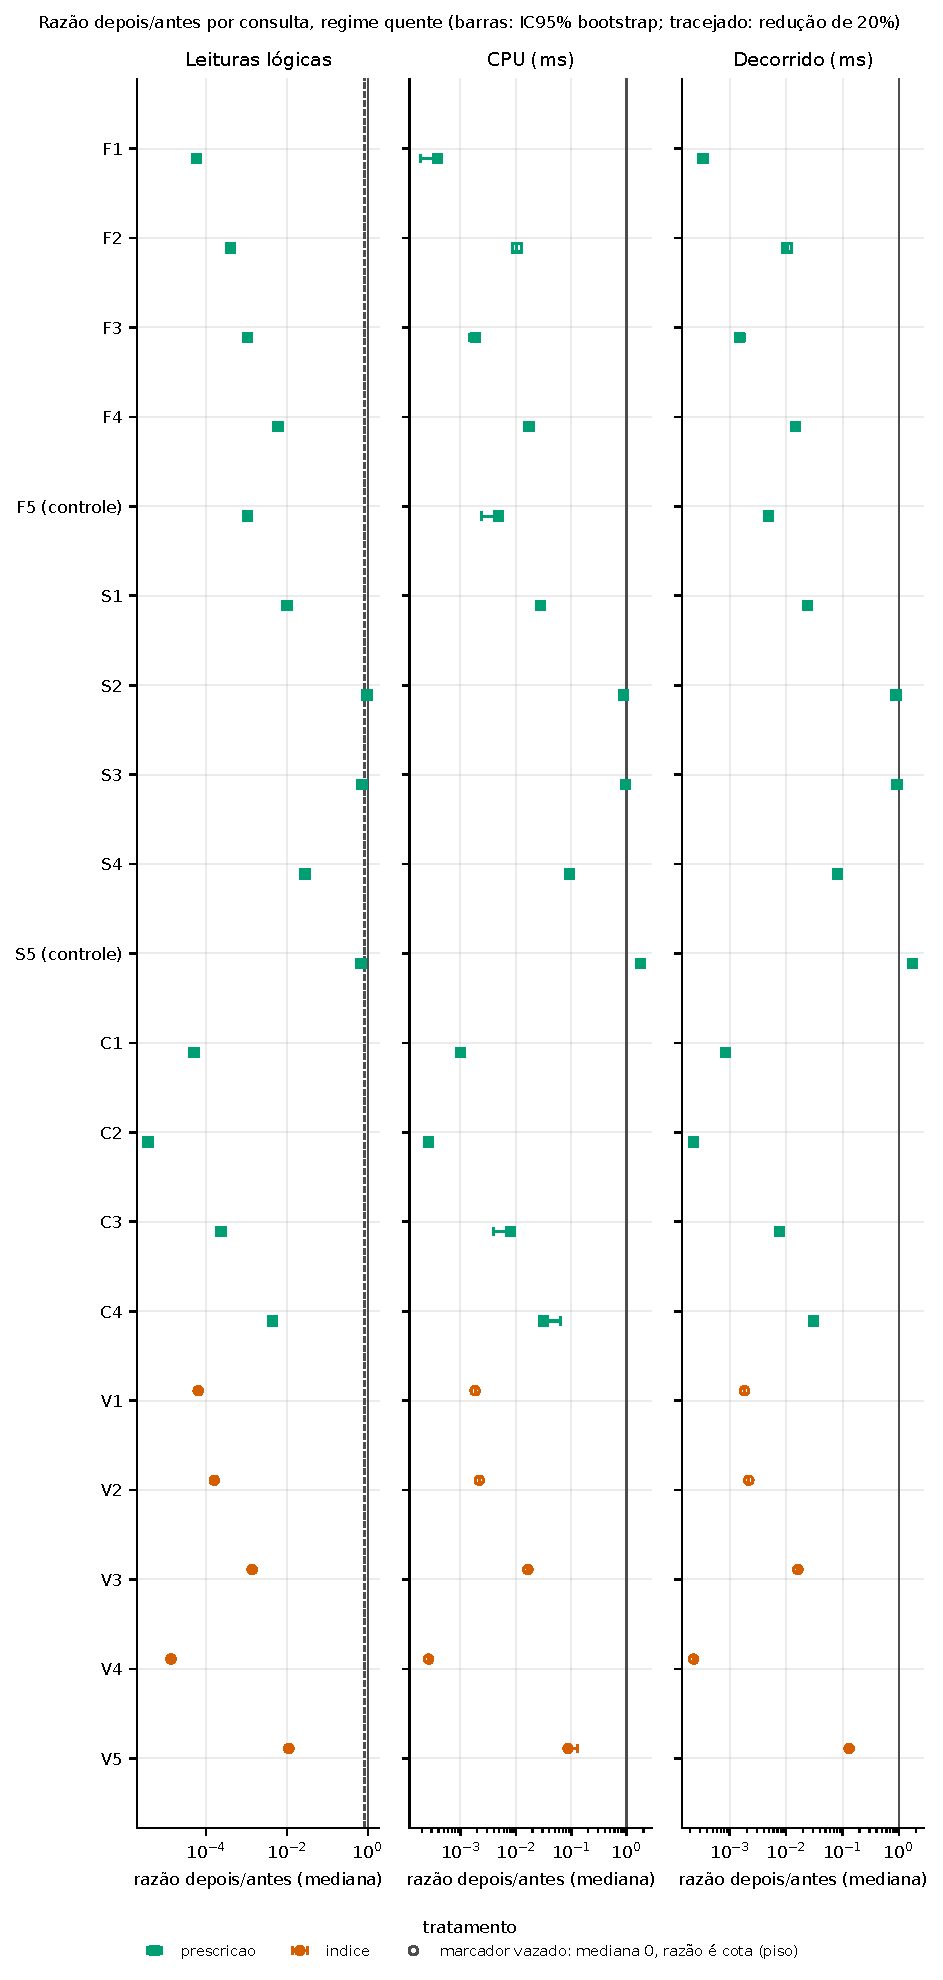
\includegraphics[width=\textwidth,height=0.78\textheight,keepaspectratio]{dados/r2/figuras/razao_por_consulta_quente.pdf}%
}{\caption{Razão entre as medições depois e antes, por consulta e métrica, cenário quente}
\label{fig:razao}}{Fonte: Do autor.}
\end{figure}

\begin{table}[H]
\centering
\flutuante{%
% gerado por gerar_tabelas_extras.py a partir de escrita-corrigida; nao editar a mao
{\footnotesize\setlength{\tabcolsep}{2.5pt}
\begin{tabular}{lrrrrrrr}
\toprule
 &  & \multicolumn{3}{c}{Leituras lógicas} & \multicolumn{3}{c}{Bytes de log} \\
\cmidrule(lr){3-5}\cmidrule(lr){6-8}
Índice & Págs. & \texttt{INS} & \texttt{UPD} & \texttt{DEL} & \texttt{INS} & \texttt{UPD} & \texttt{DEL} \\
\midrule
Badges(UserId) & 1.914 & 2,12 & 668 & 334 & 4,59 & 2,83 & 1,77 \\
Comments(PostId) +Score & 8.652 & 1,47 & 145 & 70,8 & 1,26 & 2,90 & 1,27 \\
Comments(UserId) & 6.724 & 1,18 & 137 & 69,2 & 1,86 & 2,83 & 1,26 \\
Comments(UserId) +PostId, Score & 10.560 & 1,47 & 137 & 69,2 & 1,26 & 2,96 & 1,28 \\
Comments(UserId) +4 colunas$^{\dagger}$ & 167.145 & 1,68 & 183 & 91,9 & 1,90 & 7,79 & 1,99 \\
Posts(CreationDate) & 8.330 & 1,41 & 31,6 & 15,8 & 1,06 & 2,90 & 1,07 \\
Posts(OwnerUserId) & 6.470 & 1,32 & 31,2 & 15,8 & 1,68 & 2,83 & 1,07 \\
Posts(OwnerUserId) +Score, CreationDate & 12.023 & 1,41 & 31,2 & 15,8 & 1,07 & 3,03 & 1,08 \\
Posts(OwnerUserId) +Score, ViewCount & 10.162 & 1,42 & 31,1 & 15,8 & 1,06 & 2,96 & 1,07 \\
Posts(OwnerUserId, Score) & 8.333 & 1,41 & 31,2 & 15,8 & 1,06 & 2,90 & 1,07 \\
Posts(Score, OwnerUserId) & 8.333 & 1,41 & 31,1 & 15,8 & 1,06 & 2,90 & 1,07 \\
Posts(OwnerUserId) +18 colunas$^{\dagger}$ & 863.949 & 1,76 & 41,9 & 20,5 & 1,95 & 27,7 & 1,99 \\
Users(DisplayName) +Reputation & 1.282 & 2,62 & 89,9 & 44,3 & 13,6 & 2,82 & 1,25 \\
Users(Location) & 847 & 1,29 & 85,5 & 43,3 & 1,86 & 2,98 & 1,26 \\
Users(Location) +DisplayName, Reputation & 1.772 & 2,68 & 85,5 & 43,3 & 14,1 & 3,33 & 1,30 \\
Users(Reputation) +DisplayName & 1.279 & 2,62 & 85,5 & 43,3 & 13,9 & 3,22 & 1,25 \\
Users(Location) +12 colunas$^{\dagger}$ & 7.354 & 2,60 & 85,5 & 43,3 & 18,3 & 8,56 & 2,00 \\
Votes(CreationDate) +VoteTypeId & 27.638 & 1,80 & 798 & 384 & 1,86 & 2,96 & 1,88 \\
Votes(PostId) & 17.589 & 1,61 & 798 & 384 & 1,80 & 2,83 & 1,82 \\
Votes(PostId) +CreationDate & 27.624 & 1,61 & 798 & 384 & 1,86 & 2,96 & 1,88 \\
\bottomrule
\end{tabular}\par
\vspace{3pt}
\begin{minipage}{\linewidth}\footnotesize
Razão com/sem o índice, mediana de 10 repetições de 1.000 linhas por operação (\texttt{INS} = \texttt{INSERT}, \texttt{UPD} = \texttt{UPDATE} da coluna-chave, \texttt{DEL} = \texttt{DELETE}), dentro de transação desfeita, nas mesmas linhas com e sem o índice. $^{\dagger}$ Índice sugerido pelo recurso nativo. Sem limiar de aceitação: o custo é reportado, não julgado.
\end{minipage}}
%
}{\caption{Custo de escrita por índice (razão com/sem o índice)}
\label{tab:escrita}}{Fonte: Do autor.}
\end{table}
 % Apêndice A (depois das referências, ABNT)


\end{document}
